\documentclass[brazil]{abnt}
\usepackage[utf8]{inputenc}
\usepackage[brazil]{babel}
\usepackage{listings}

\usepackage{courier}
 \lstset{
         basicstyle=\footnotesize\ttfamily, 
         numberstyle=\tiny,          
         numbersep=5pt,              
         tabsize=2,                  
         extendedchars=true,         
         breaklines=true,            
         keywordstyle=\color{red},
                frame=b,         
         stringstyle=\color{white}\ttfamily, 
         showspaces=false,           
         showtabs=false,             
         %xleftmargin=17pt,
         %framexleftmargin=17pt,
         %framexrightmargin=5pt,
         %framexbottommargin=4pt,
         %backgroundcolor=\color{lightgray},
         showstringspaces=false      
 }
 \lstloadlanguages{
         %[Visual]Basic
         %Pascal
         %C
         C++,
         XML
         %HTML
         %Java
 }

\usepackage{color}
\usepackage{xcolor}
\usepackage{graphicx}
\usepackage{wrapfig}
\usepackage{xunxos-utp}
\usepackage{caption}
\DeclareCaptionFont{white}{\color{white}}
\DeclareCaptionFormat{listing}{\colorbox{gray}{\parbox{0.98\textwidth}{#1#2#3}}}
\captionsetup[lstlisting]{format=listing,labelfont=white,textfont=white}


\makeatletter
\usepackage{babel}
\makeatother
\begin{document}

\autor{Renato dos Santos Cerqueira}
\coautor{Felipe Pedrosa Martinez}
\titulo{Ferramentas e métodos para o desenvolvimento de um jogo de plataforma 2D para o Nintendo DS}
\orientador{Adriano Joaquim de Oliveira Cruz}
\comentario{Monografia apresentada para obtenção do Grau de Bacharel em Ciência da Computação pela Universidade 
Federal do Rio de Janeiro.}
\instituicao{Departamento de Ciência da Computação \par Instituto de Matemática \par Universidade Federal do Rio de Janeiro}
\local{Rio de Janeiro - RJ, Brasil}
\data{13/07/2011}

\Ncapa
\NFolhaDeRosto

%\begin{folhadeaprovacao}
%Monografia de Projeto Final de Graduação sob o título \textit{``\ABNTtitulodata''},
%defendida por \ABNTautordata~e \ABNTcoautordata~e aprovada em \ABNTdatadata, no Rio de Janeiro,
%Estado do Rio de Janeiro, pela banca examinadora constituída pelos
%professores: \setlength{\ABNTsignthickness}{0.4pt}

%\assinatura{Prof. Ph.D. Adriano Joaquim de Oliveira Cruz\\ Orientador} \assinatura{???\\ Universidade ???} \assinatura{???\\ Universidade ???}
%\end{folhadeaprovacao}

\begin{resumo}
O objetivo deste trabalho é fazer um \textit{engine} de jogo para o \textit{videogame Nintendo DS\texttrademark} e também um editor de fases 
e configurações, como seria feito numa equipe de desenvolvimento de um jogo comercial, dando a possibilidade aos \textit{designers} 
de fazerem seus \textit{sprites} e criarem as fases com eles, sem que fosse necessário mexer com códigos.
\end{resumo}

\begin{abstract}
The objective of this paper is to make a game engine to the Nintendo DS\texttrademark system and a level and configurations editor, as it
would be done in a development team in a comercial game, giving designers the possibility to make their sprites and create their levels 
without touching actual source code.
\end{abstract}

\chapter*{Dedicatória}

\chapter*{Agradecimentos}

\tableofcontents{}
\listoffigures
%\listoftables

\chapter{Introdução\label{cap:introducao}}

\vfill{}
\begin{flushright}{}``\emph{Quote 1}''\\
{\small Author1}\end{flushright}{\small \par}
\vfill{}

Neste capítulo são apresentados o objetivo desta monografia e a estrutura da mesma.
\newpage


\section{Objetivo deste trabalho}

A área de jogos eletrônicos é uma área relativamente nova, se comparada a outros ramos da ciência da computação. No entanto, por mais que a área de jogos compreenda conceitos importantes de computação, ela engloba outros que fogem ao seu escopo. Nesse sentido, para o desenvolvimento de um jogo eletrônico, além de conhecimentos de linguagens de programação, algoritmos e estruturas de dados, interface humano-computador e inteligência artifical, é preciso considerar também os aspectos subjetivos que dizem respeito a um jogo de forma geral, seja ele eletrônico ou não. O gameplay, ou a mecânica do jogo, ou seja, a forma com que o jogo vai se desenrolar e o seu funcionamento, é um exemplo claro de que o seu desenvolvimento e sua concepção vão muito além do que pode ser programado, compilado e executado em um computador.

É possível observar o crescimento da área de jogos eletrônicos se notarmos que o primeiro exemplo conhecido aparece em 1947, quando Thomas T. Goldsmith Jr. e Estle Ray Mann introduziram sua patente para um Dispositivo de Entretenimento usando Tubo de Raios Catódicos em \cite{2455992}. 

Com a tecnologia cada vez mais aprimorada, conceitos básicos que definiam os jogos daquela época vêm sido substituídos por formas cada vez mais rebuscadas. Novos elementos de jogabilidade vêm sido incorporados à mecânicas clássicas, e estas evoluem por si só, dadas as cada vez menores limitações e as constantes inovações de hardware e interação com o jogador. Isso tudo se reflete no desenvolvimento de novas áreas de jogos: onde antes havia poucos estilos bem definidos, como corrida, luta e aventura, encontramos novos nichos como por exemplo jogos casuais, sociais e de multiplay massivo.

Jogos produzidos na época do Atari 2600 e Magnavox Odyssey, por exemplo, eram criações de um único desenvolvedor e em geral, concluídos em períodos curtos de tempo, sem nem ao menos identificá-lo. Em razão disso, era comum a aparição de \textit{Easter Eggs}, recursos que os desenvolvedores utilizavam para assinar a sua criação, mesmo que de uma forma não convencional \cite{PrimeiroDevName}.

Hoje em dia, a indústria de jogos conta com super-produções que com uma quantidade quase infindável de desenvolvedores, designers, criadores de fases, dentre outros tantos profissionais trabalhando cada um com sua especialidade.

Neste trabalho, pretendemos nos inserir no contexto desses times de criação, sob a ótica do desenvolvedor, que, através da criação de ferramentas, facilita a interação entre as demais equipes do time de desenvolvimento.

Assim, criaremos um jogo em duas dimensões, do tipo plataforma para o videogame portátil Nintendo DS. Para isso, desenvolvemos uma \textit{engine}, responsável por controlar todas as partes envolvidas no funcionamento do jogo como áudio, vídeo, estruturas de dados, controle de personagens, fases e itens.

Parte do nosso objetivo foi tornar esta \textit{engine} simples e de fácil reutilização. Isto foi feito através de ferramentas de criação e configuração dos componentes pertinentes ao mundo do jogo.

%Faremos o papel do desenvolvedor: Criar as ferramentas, imaginando como os outros times as usariam e aprimorando-as ao máximo para esse fim.

\section{Contextualização}

Conforme dito anteriormente, criaremos ferramentas para desenvolver jogos em duas dimensões do tipo de plataforma. O questionamento imediato a partir desta proposta é: o que é exatamente um jogo de plataforma em duas dimensões?

Basicamente, estes são jogos onde a movimentação do personagem principal se dá verticalmente ou horizontalmente, sem considerar a aproximação ou o distanciamento deste ao jogador. Conforme o personagem se desloca pelo mundo, este vai se revelando a ele, e é comum que apresente inimigos e obstáculos, como uma fileira de espinhos ou buracos sem fundo. Em geral, o personagem principal tem um objetivo que o motiva a atravessar o mundo que o é apresentado, podendo ou não saltar ou possuir alguma habilidade especial, ter ou não acesso a alguma arma ou item, e enfrentar algum grande inimigo no final de tudo. Esta é uma definição bastante aberta, e é nela que nos inspiramos para escrever o \textit{engine} que será executado no Nintendo DS. Para ilustrar, podemos pensar em exemplos clássicos, como Super Mario World para o Super Nintendo, ou Sonic The Hedgehog para o Sega Mega Drive. É certo que nem todos os jogos plataforma são em duas dimensões. Entretanto, neste trabalho, o foco será exclusivamente nos jogos de plataforma em duas dimensões, para facilitar o entendimento e o desenvolvimento de soluções.

Nessa modalidade de jogos, um recurso muito utilizado pelos desenvolvedores são \textit{tiles} - ladrilho, em inglês - figuras de tamanho pré-definido, que compõem todo o mundo. Além disso, nesse tipo de jogo, todos os objetos costumam ser feitos a partir da combinações de \textit{sprites}, usados mais de uma vez e em diferentes posições. Os \textit{sprites} são responsáveis por representar possiveis inimigos, por exemplo. De forma mais simples, é possível dizer que enquanto os \textit{tiles} compõem o mundo, os \textit{sprites} o habitam.

Dentro desse contexto, o objetivo é criar uma \textit{engine} que leia um arquivo de configuração, onde estarão detalhadas informações sobre quais são as imagens que compõem o personagem principal (ou personagens, no caso de haver uma escolha); informações sobre os inimigos (como por exemplo a qual tipo de movimento que cada um obedece); descrição dos itens (como qual efeito ele causa no personagem principal ou nos inimigos) e informações sobre as fases (dentre elas o posicionamento dos elementos que as compõem).

\section{Estrutura da monografia}

Escrever aqui a estrutura da monografia.

\chapter{Desenvolvendo para o Nintendo DS\label{cap:hardds}}

\vfill{}
\begin{flushright}{}``\emph{Quote 2}''\\
{\small Author 2}\end{flushright}{\small \par}
\vfill{}

Neste capítulo são apresentados a motivação para desenvolver para a plataforma, as suas especificações e como desenvolver.
\newpage

\section{Motivação}

Há poucos trabalhos desenvolvidos para plataformas diferentes do PC, seja pelo mais restrito número de usuários, menor versatilidade de ferramentas e recursos associados ou mesmo pela maior dificuldade de encontrar documentação relativa ao desenvolvimento. A motivação para este trabalho é, dadas essas circunstâncias, criar um facilitador para o desenvolvimento de jogos para um console real, desenvolvendo ferramentas para fomentar uma maior quantidade de trabalhos para a plataforma, apesar das dificuldades.

\section{Especificações}

O foco deste trabalho se dá nas duas primeiras iterações do Nintendo DS: o Nintendo DS original, lançado no final de 2004, que normalmente é chamado de ``DS Phat''; e sua segunda iteração, o Nintendo DS Lite, lançado no meio de 2006.

Ambos possuem um hardware muito parecido, sendo as suas maiores diferenças a estética, o contraste e iluminação da tela. Nesta seção, são detalhadas as especificações de cada um:

\noindent{\bf Nintendo DS:}\\
{\bf Peso:} 275 gramas\\
{\bf Dimensões:} 148.7mm x 84.7mm x 28.9mm\\
{\bf Telas:} Duas telas, ambas com 3 polegadas, de LCD TFT (\textit{Thin-Film Transistor}) com 18-bit de cor, resolução de 256x192. As duas telas tem um espaço entre elas de aproximadamente 21mm. A tela inferior possui \textit{touchscreen} resistivo, que responde a um ponto de pressão por vez. No caso de vários pontos da tela serem pressionados simultaneamente, ela responde na posição média destes pontos.\\
Além disso, a tela possui iluminação traseira, que pode ser desligada por software.\\
{\bf Entradas:} Duas entradas de cartucho, uma para o formato de cartucho do seu antecessor, o Gameboy Advance(GBA), na parte inferior,e uma para seu próprio formato de cartucho na parte superior.\\
{\bf Processadores:} Dois processadores ARM, um ARM946E-S a 67MHz, que é o processador principal, responsável pelo \textit{loop} de jogo e renderização de vídeo e um coprocessador ARM7TDMI a 33MHz, responsável pelo som, wi-fi, e que quando em modo GBA, diminui seu \textit{clock} para 16MHz, e passa a ser responsável pelo processamento principal.\\
{\bf Memória:} 4MiB de RAM principal, expansíveis através da entrada de Gameboy Advance. No entanto, essa expansão só foi usada em jogos oficiais pelo Opera Browser.\\
{\bf Wireless:} Conexão IEEE802.11b, compatível com encriptação por WEP. WPA e WPA2 não são suportadas. Essa conexão também pode ser usada para comunicação entre consoles.\\

\noindent{\bf Nintendo DS Lite:}\\
{\bf Peso:} 218 gramas\\
{\bf Dimensões:} 133mm x 73.9mm x 21.87mm\\
{\bf Telas:} Mesma especificação que o original, no entanto, possui quatro níveis de iluminação que podem ser reguladas por software. A tela também possui um contraste melhor que o original.\\
Existem algumas outras menores diferenças, como a mudança do chip que controla o \textit{Wireless}, o controlador da \textit{touchscreen} também é ligeiramente diferente, mas para fins práticos, o resto da configuração é igual ao original.

\section{Desenvolvimento}

O desenvolvimento oficial no DS segue os mesmos moldes do desenvolvimento em consoles diversos: a Nintendo possui um time interno chamado de Intelligent Systems Co. Ltd. responsável pelas ferramentas de desenvolvimento para os consoles da empresa, dentre eles, o Nintendo DS. De outro lado, desenvolvedores independentes ou empresas de desenvolvimento, interessados em criar jogos para o console, pode entrar em contato com a empresa em busca das ferramentas necessárias, que incluem uma unidade especial de desenvolvimento, que se conecta ao computador por meio de uma porta USB. Justamente por ser voltada para desenvolvimento, dentre outras particularidades, esta unidade possui o dobro de memória de uma unidade normal, de forma a facilitar o Debug. No entanto, para adquiri-las, é necessário assinar um Acordo de Confidencialidade (do inglês, \textit{Non-Disclosure Agreement}), que não permite que se comente ou escreva sobre esses \textit{kits} de desenvolvimento. Por causa disto, é difícil encontrar mais detalhes acerca de seu funcionamento.

\begin{figure}
\centering
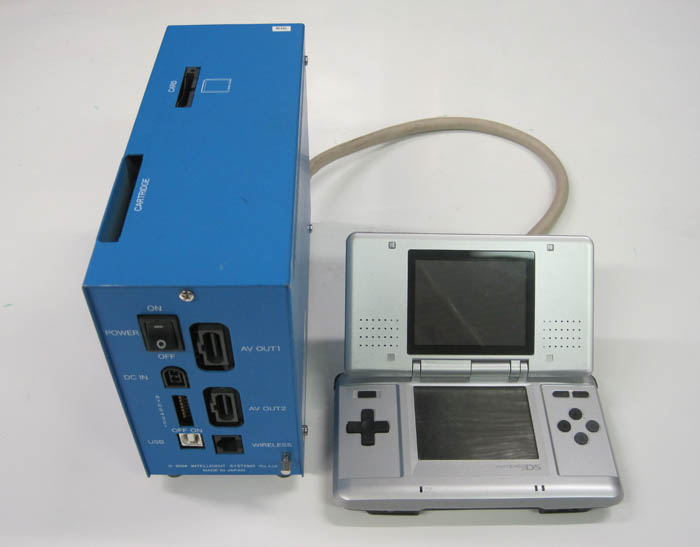
\includegraphics{imgs/is_devkit1.jpg}
\caption{Uma imagem do kit de desenvolvimento oficial do Nintendo DS original} 
\end{figure}

Em geral, pequenas empresas de desenvolvimento não têm acesso ao \textit{kit} de desenvolvimento oficial, seja por causa dos altos custos para obter o hardware ou pela dificuldade de adquirir as licenças. Desta forma, a publicação de jogos para consoles do tipo ainda é rara no mercado atual de jogos.

Para os fins do presente trabalho, cabe recorrer ao desenvolvimento não oficial, apelidado de \textit{Homebrew}. A cadeia de ferramentas usada é chamada devkitArm, que serve para compilar programas em C e C++ para consoles com processadores ARM. Ao contrário do desenvolvimento oficial, não é possível produzir cartuchos de jogos \textit{Homebrew}. Para testarmos, no entanto, podemos fazer uso de emuladores ou de um Nintendo DS com uso de um \textit{flash cartridge}, um cartucho que possui uma memória \textit{flash}, como um \textit{pendrive}, e que pode ser apagada e reescrita várias vezes. Este cartucho não é suportado pela Nintendo.

A partir do devkitArm, foi desenvolvida a biblioteca libnds, feita especificamente para o hardware do DS. Essa biblioteca inclui funções de baixo nível que acessam todo o hardware: som, video, \textit{wireless}, controle, dentre outros. O desenvolvimento nela apresenta dificuldades dado o baixo nível de suas instruções. Muitas vezes é necessário o uso de endereços de memória, cópias diretas da memória principal para a memória de vídeo, dentre outros artifícios não usuais na programação atual. Dado este cenário, baseadas na libnds, surgiram algumas bibliotecas em um nível mais alto. Para o desenvolvimento deste trabalho, foi escolhida a PALib, uma biblioteca que visa facilitar o desenvolvimento de jogos em duas dimensões que usem \textit{sprites} e mapas de fundo.

Ainda assim, o uso dessas ferramentas não é trivial. Diferente de um programa convencional para desktop, as suas funcionalidades se apresentam em formas menos claras para o desenvolvedor: incluir ou gerar imagens, por exemplo, implica em um fluxo de trabalho diferente do esperado por um time de desenvolvimento convencional. 

O conjunto de ferramentas desenvolvidos neste trabalho tem como objetivo tornar mais transparente e intuitivo o desenvolvimento no cenário apresentado. As ferramentas desenvolvidas são, em sua maioria, visuais para que o seu uso se dê de uma forma simplificada.

% escrevi esse parágrafo sobre QT, mas ele provavelmente precisa de uma revisada.

Para desenvolver as ferramentas foi usado o QT, um \textit{Framework} multi-plataforma que permite o uso de interfaces gráficas em C++, além de possuir classes que facilitam o acesso a tecnologias como XML, acesso a diversos formatos de arquivos de imagem, dentre outras possibilidades. A escolha foi feita para que as ferramentas funcionem em diversos sistemas operacionais sem precisar de mudanças no código.

\chapter{As Ferramentas\label{cap:ferramentas}}

\vfill{}
\begin{flushright}{}
\begin{figure}[h!]
\hfill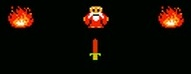
\includegraphics{imgs/oldman.jpg}
\end{figure}
``\emph{It's dangerous to go alone! Take this.}''\\
{\small Old Man (Zelda)}\end{flushright}{\small \par}
\vfill{}

Neste capítulo são apresentadas as ferramentas e o seu método de uso.
\newpage

\section{A criação do jogo\label{sec:workflow}}

Um jogo necessita de algumas partes constituintes, como por exemplo, suas fases e cenários, seus itens, inimigos e personagem principal. Com o uso das ferramentas apresentadas neste trabalho, o usuário executa os seguintes passos:

Em primeiro lugar, o usuário cria os cenários usando a BGTool, onde ele desenha os cenários em que o jogo vai se passar. Esses cenários ficam organizados logicamente em fases, e essas fases, no produto final, aparecerão encadeadas.

Em seguida, é necessário importar as figuras dos personagens, inimigos e itens. Isso é feito a partir da SpriteTool. 
%\footnote{Precisamos pensar em como juntar as duas coisas. Como o usuário posiciona inimigos e itens no cenário? Há uma terceira ferramenta? Fazemos uma das duas ferramentas fazerem isso, adicionalmente?}

\section{BGTool: A ferramenta de criação de cenários}

A BGTool foi criada com o objetivo de permitir que o usuário importe seus \textit{tiles} pré-existentes e a partir deles, desenvolva um novo cenário. Além disso, a ferramenta também é responsável por exportar esse cenário para o formato do Nintendo DS. 

Ao começar um novo projeto, o usuário pode escolher quantas camadas de \textit{background} o cenário que está sendo criado terá. O hardware do DS suporta até cinco camadas de \textit{background}, no entanto, usar todas elas não é compulsório e o número de camadas a serem usadas fica a critério do desenvolvedor. Com as várias camadas, porém, a gama de recursos para o desenvolvimento do jogo aumenta significantemente. O desenvolvedor pode, por exemplo, fazer uso de Paralaxe, uma técnica em que as camadas mais distantes da câmera se movem mais devagar, dando uma ilusão de profundidade e imersão.

Por uma combinação de exigências do hardware do DS e das bibliotecas usadas, uma camada de \textit{background}, na verdade, é implementada como um mapa de \textit{tiles}. Isto significa dizer que as imagens que compõem o \textit{background} são compostas de imagens menores, de tamanho fixo, que podem ou não ser rotacionadas ou espelhadas na vertical ou horizontal. E estas imagens menores são chamadas de \textit{tiles}, conforme mostrado anteriormente.

Portanto, além do número de camadas, o usuário também especifica o tamanho dessas. A única limitação quanto ao seu tamanho é ter suas dimensões múltiplas de 8. Assim, neste trabalho, utilizamos \textit{tiles} de tamanho 8x8 pixels, o mais simples de ser utilizado no DS.

\begin{figure}[h!]
\centering
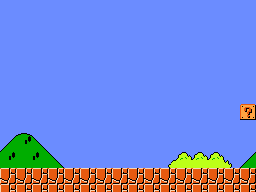
\includegraphics[scale=1]{imgs/exemplo.png}
\caption{A imagem antes de ser carregada} 
\end{figure}

\begin{figure}[h!]
\centering
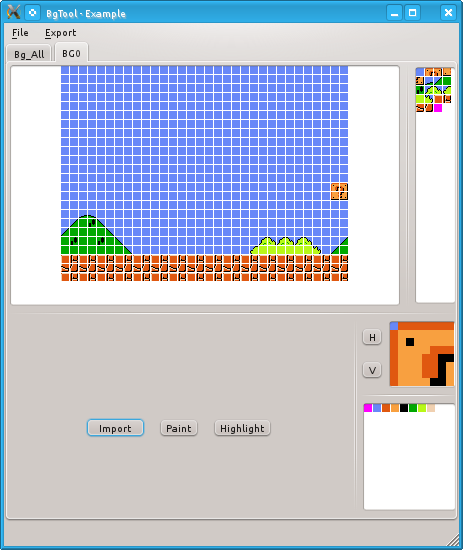
\includegraphics[scale=1]{imgs/bgtool1.png}
\caption{A imagem após a abertura na ferramenta} 
\end{figure}

Ao importar os \textit{tiles}, o usuário pode usá-los para editar o \textit{background} da fase que está construindo. Uma paleta é gerada automaticamente pela ferramenta a partir dos \textit{tiles} que o usuário carrega. Em seguida, a ferramenta se encarrega de fazer a importação de uma imagem e transformá-la em \textit{tiles}, dividindo-a em partes de 8x8 pixels e eliminando as possiveis repetições. Como o DS suporta espelhamento na horizontal e na vertical de um \textit{tile}, então é feita uma verificação se o \textit{tile} em questão é igual a um dos \textit{tiles} existentes, em quaisquer das configurações: sem espelhamento, com espelhamento vertical, horizontal ou ambos.

Os \textit{tiles} são armazenados como imagens, sendo assim não há um algoritmo de \textit{hash} disponível no QT que pudesse ser utilizado para organizá-los. A implementação de tal algoritmo foge ao escopo deste trabalho e por isso, é feita uma busca exaustiva pelo vetor de imagens comparando as imagens geradas com as que já existem. Embora esse seja um processo relativamente custoso, com complexidade O(n) para cada inserção, dado o tamanho da entrada de dados, este custo pode ser ignorado.

\begin{figure}[h!]
\centering

\includegraphics[scale=1]{imgs/tiles1.png}
\caption{Alguns \textit{tiles} depois de separados} 
\end{figure}

\begin{figure}[h!]
\centering

\includegraphics[scale=1]{imgs/tiles2.png}
\caption{Configurações possíveis para um \textit{tile}} 
\end{figure}

Com os \textit{tiles} já importados, o usuário pode construir os mapas que compõem a fase. A ferramente separa as diversas camadas de fundo em abas, para a edição separada de cada uma. Porém, ao construir uma fase, é possível ver uma composição destas camadas em uma imagem de \textit{background} de forma a prover um \textit{feedback} do ao usuário de como ficaria a versão final da fase.

Ao salvar o projeto, guardamos suas informações num arquivo XML com um formato bem definido, numa área delimitada destinada à BGTool. Lá, ficam organizadas informações relativas às diversas fases tais como suas camadas. Isto será explicado com mais detalhes na seção \ref{sec:xml}.

A qualquer momento, o usuário pode exportar o que já está pronto para o DS, esse é um processo transparente em que criamos os arquivos necessários para a execução da fase criada pelo usuário. São criados três arquivos, um arquivo Pal, que contém a paleta, um arquivo Tile que contém os \textit{tiles}, indexados pela paleta e um arquivo Map, que contém o mapa, ou \textit{background}, indexado pelos \textit{tiles}.
 
Os três arquivos são binários e obedecem a um formato delimitado pela PALib e suas funções que coordenam o carregamento de cenários.

Uma breve explicação desses formatos é a seguinte:

\begin{itemize}
 \item Arquivo Pal\\
 Neste arquivo, temos informações sobre a paleta usada no arquivo. São descritas todas as cores contidas no arquivo. Precisam haver 256 cores, mesmo que o arquivo seja inflado de cores falsas. O Formato usado no arquivo é A1B5G5R5, o que significa que há um bit para o caso da cor ser transparente (alpha channel), 5 para o verde, 5 para o azul e 5 para o vermelho. A primeira cor no arquivo é a cor usada como transparência. (A cor padrão sendo o Magenta)\label{exp:A1B5G5R5}
 \item Arquivo Tiles\\
 Neste arquivo, ficam os \textit{tiles}, cada um de 8x8 pixels. Cada pixel do \textit{tile} referencia uma cor do arquivo Pal. Neste arquivo, os tiles são escritos em blocos (vetores) de 64 bits. 
 \item Arquivo Map\\
 Neste arquivo, fica o mapa do \textit{background}, ele referencia os tiles. Os bits 0-9 indicam o tile, o bit 10 indica se é espelhado na horizontal e o bit 11 indica se é espelhado na vertical. Os bits restantes indicam qual paleta está sendo usada para o mapa em questão, eles não são usados nos modos em que só há uma paleta, ou seja, modos de 256 cores.
 \item Arquivo .c\\
 Este arquivo constrói a struct que será usada no programa, informa o tipo do mapa, o seu tamanho, os ponteiros para as regiões onde ficaram os três arquivos acima depois de linkados, tamanho do tiles em bytes e tamanho do mapa em bytes. 
\end{itemize}

No momento em que o usuário carrega uma imagem, ela é convertida para um formato de 256 cores. Devido as limitações de cor, o ideal seria que o usuário já carregasse imagens com apenas 256 cores, desta forma não há perda ou alteração de cores da imagem original, ou no caso dessa perda ser necessária, ela acontece com o controle do usuário.

Pelo mesmo motivo, caso mais de uma imagem seja utilizada na composição de um mapa, o usuário deve fazer com que as imagens compartilhem uma mesma paleta.

Depois dessa conversão inicial, todas as ações no programa são feitas usando a paleta gerada na fase de carregamento. Na exportação, a paleta é exportada diretamente, sendo simplesmente colocada no arquivo binário.

Os \textit{tiles}, quando exportados, também não necessitam de preocupação adicional. Sua conversão para o formato binário envolve apenas obter o indice da cor de cada pixel de cada \textit{tile} e escrevê-lo no arquivo binário.

A geração do mapa, ou \textit{background}, é a tarefa mais complexa. Internamente na ferramenta, o mapa é armazenado como uma matriz de estruturas do tamanho do cenário, onde cada estrutura armazena o índice do \textit{tile} daquela posição e também se naquela posição este tile está espelhado na vertical, na horizontal ou ambos. 

Obtidas essas informações, fazemos uma conversão para o formato discutido acima e exportamos para o arquivo binário.

\lstinputlisting[caption=Função que exporta o mapa,label=list:exportmap]{codigos/exportmap.cpp}

Por fim, depois de exportados, esses arquivos estarão prontos para serem usados num estágio posterior da cadeia de desenvolvimento e inseridos no jogo final.

\section{SpriteTool: A ferramenta de criação de \textit{sprites}}

A SpriteTool foi criada com o objetivo de, a partir de simples imagens, gerar \textit{sprites} para o desenvolvimento de um jogo completo, executável no Nintendo DS. O objetivo de tal ferramenta é criar um ambiente para o usuário, no qual ele não tenha que lidar com as particularidades do desenvolvimento que não sejam pertinentes à criação do \textit{sprite} em si.

Além de permitir a portabilidade das imagens para o Nintendo DS, transformando-as em \textit{sprites} do jogo no formato reconhecido pelo console, a SpriteTool gera um arquivo de projeto no formato XML, que pode ser reconhecido pelas outras ferramentas desenvolvidas neste trabalho. A integração entre estas ferramentas é feita respeitando protocolos pré-estabelecidos de escrita e leitura nestes arquivos, de forma transparente para o usuário. A seção \ref{sec:xml} aborda em detalhes a estrutura do formato escolhido e como cada uma das ferramentas faz uso dele para armazenar e resgatar as informações pertinentes ao desenvolvimento do jogo.

\begin{figure}[h!]
\centering
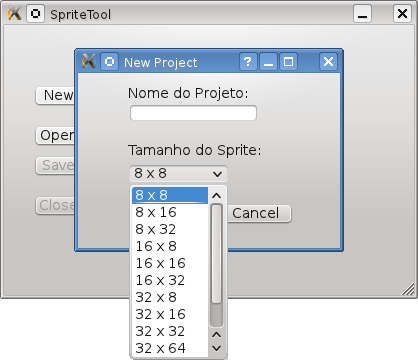
\includegraphics{imgs/spritetool1.png}
\caption{Janela de criação de novo \textit{sprite}} 
\end{figure}

Ao começar um novo projeto, uma instância de \textit{sprite} é criada, mesmo que ainda não tenha sido adicionada nenhuma imagem. É importante salientar que o termo “Sprite” neste escopo, engloba uma série de conceitos que vão além de um simples arquivo de imagem. São eles: informações relativas ao tamanho da imagem, uma paleta de cores, informações sobre transparência e, por fim, os \textit{frames} do \textit{sprite} – que são as imagens em si.
Algumas destas informações são requeridas para a criação do projeto de \textit{sprite}, como o nome do \textit{sprite} e as dimensões das imagens que servirão como \textit{frames} da animação deste. O programa oferece uma gama de formatos de \textit{sprite} para o usuário escolher, respeitando as restrições das bibliotecas e do hardware do DS sobre as imagens que podem ser usadas como \textit{sprites}.

Criado um novo projeto de \textit{sprite}, o usuário tem a possibilidade de adicionar novas imagens a ele. Além de permitir que o usuário busque uma imagem compatível com o tamanho já definido, o programa cria uma pasta de projeto e mantém nesta pasta uma cópia de cada imagem adicionada a ele, eliminando o uso de caminhos específicos para os arquivos fontes das imagens selecionadas. Assim, o programa tem uma maior portabilidade de uso. De forma análoga, as imagens relativas aos \textit{frames} deletados do projeto são removidas desta pasta que encapsula apenas os arquivos necessários para o funcionamento do SpriteTool.

Com a ferramenta, ainda é possível pré-visualizar a animação do \textit{sprite}, provendo ao usuário uma ideia do comportamento do \textit{sprite} dentro do jogo. Ainda que esta  visualização não ofereça suporte aos eventos normalmente associados com cada parte da animação, como por exemplo o personagem pular ao ser apertado o botão de pulo, ela é um \textit{feedback} importante para a definição da animação, permitindo verificar o quão fluídos os movimentos do personagem estão. **

Depois de adicionar as imagens que vão compor o \textit{sprite} e de validar o resultado da animação, o fluxo de trabalho para o usuário termina salvando o projeto e exportando para o formato compatível com as especificações de \textit{sprite} do Nintendo DS e da PALib. Todo o processamento feito ao executar estas duas funções é transparente a ele. 

Ao exportar, o SpriteTool traduz as informações do \textit{sprite} para o formato que poderá ser usado no desenvolvimento do jogo dentro da \textit{engine}. Para que isto aconteça, são necessários dois arquivos: nomedoprojeto\_Pal.bin e nomedoprojeto\_Sprite.bin

O primeiro arquivo contém as informações relativas à paleta de cores daquele \textit{sprite}. Isto deve ser feito para cada \textit{frame} contido no projeto, da seguinte forma:

Como o formato de cor aceito pelo Nintendo DS é o formato A1B5G5R5, citado em \ref{exp:A1B5G5R5}, a cor de cada pixel da imagem é pré-processada de forma a se adequar ao padrão. Depois disso, é preciso verificar se a cor já existe na paleta que está sendo criada. Para tal, é feito o uso de uma tabela \textit{hash} tanto pela sua praticidade quanto pelo seu desempenho. Se a cor ainda não existe na paleta ela é adicionada. Vale ressaltar que por convenção, a cor magenta representa a transparência e é a primeira cor a ser adicionada na paleta. 

Após o processamento de todos os \textit{frames} do projeto, o arquivo nomedoprojeto\_Pal.bin está completo e pronto para uso na \textit{engine}.

O segundo arquivo que é gerado nesta etapa, contem as informações referentes aos \textit{frames}. Nele é descrito como cada \textit{frame} é organizado, baseando-se nos índices das cores referenciadas na paleta do projeto. O formato no qual isto deve ser feito, exige que o programa itere os \textit{frames} em blocos de 64 pixels (8 de altura por 8 de largura). O fim do processamento se dá junto ao término dos \textit{frames} do projeto de \textit{sprite}. 

Com estes dois arquivos criados, a \textit{engine} é capaz de reconhecer o \textit{sprite} e animá-lo conforme conveniente. 

\lstinputlisting[caption=Exportando o \textit{sprite} para o Nintendo DS:,label=list:exportsprite]{codigos/listingexportsprite.c}

Para o desenvolvimento desta etapa, foi usado um editor hexadecimal de forma a facilitar a visualização dos arquivos gerados pela ferramenta e verificar a resposta que eles tinham na \textit{engine}.

\section{A integração entre as ferramentas\label{sec:xml}}

As ferramentas desenvolvidas neste trabalho têm como objetivo conjunto possibilitar o desenvolvimento de jogos no Nintendo DS. Estas ferramentas foram desenvolvidas de forma separada, cada uma sendo responsável por uma parte específica da cadeia de desenvolvimento. Desta forma, se faz a necessário estabelecer um meio de comunicação entre elas. É importante ressaltar que esta forma de comunicação deve ser robusta, para que permita, por exemplo, uma integração futura entre as ferramentas apresentadas neste trabalho, construindo assim um único ambiente de desenvolvimento. 

Além disso, seja para fins de interromper momentaneamente o fluxo de trabalho em uma determinada etapa do desenvolvimento, ou guardá-lo para referência futura, fez-se necessário, também, estabelecer um meio de armazenamento da informação usada por cada uma das ferramentas.

Para resolver estas questões, foi escolhido o formato de arquivo XML como um meio intermediário entre as ferramentas, sendo responsável tanto para armazenar informações de configuração de cada uma delas, quanto para estabelecer uma possível comunicação entre elas. Este formato é amplamente usado hoje em dia e foi escolhido pela facilidade de uso e legibilidade que traz consigo. 

Os arquivos XML são compostos por diversas \textit{tags}, responsáveis por delimitar um determinado espaço no arquivo onde se encontra a informação referente a ela. Dentro da área delimitada por uma \textit{tag}, existe a possibilidade de criarmos mais um nível de profundidade no arquivo, estabelecendo assim um sistema hierárquico dentro dele. Dessa forma, este tipo de arquivo pode ser entendido como uma árvore, onde cada \textit{tag} representa um nó, e cada nível hierárquico abaixo dele representa um filho. Isto traz a vantagem de introduzir diferentes ramos, cada um contendo um tipo específico de informação, todos no mesmo arquivo. Assim, ferramentas distintas têm suas informações completamente separadas, mas todos os dados relativos a um mesmo projeto se encontram no mesmo arquivo. 

Depois de escolhido o formato XML, foi criado um protocolo de escrita e leitura a ser respeitado por todas as ferramentas.

\lstinputlisting[caption=Formato de XML de integração entre as ferramentas,label=list:xml]{codigos/exemplo.xml}

\chapter{A Engine}

\vfill{}
\begin{flushright}{}``\emph{Quote 4}''\\
{\small Author4}\end{flushright}{\small \par}
\vfill{}

Neste capítulo é apresentada a \textit{engine} feita para o Nintendo DS e as decisões tomadas sobre ela.
\newpage

\section{Introdução}

No capítulo anterior foi demonstrado como este trabalho resolve a primeira parte do processo de criação do jogo: a criação de seus personagens e \textit{backgrounds}. Ficam então alguns desafios pela frente: a detecção de colisão, a constituição do mundo e a interligação das fases, isto é, o próprio desenrolar do jogo.

Para resolver esses desafios, se faz necessária a criação de alguma ferramenta no Nintendo DS. Não é a intenção deste trabalho apresentar uma \textit{engine} completa, no entanto, é pretendido se criar uma espécie de \textit{engine} que consiga usar-se dos personagens e \textit{backgrounds} criados com as ferramentas previamente apresentadas.

Podemos estabelecer que a \textit{engine} criada é, na verdade, um template, que pode (e deve) ser modificado pelo programador para torná-la adequada ao jogo em desenvolvimento.

\section{O \textit{Loop} de jogo}

Podemos encontrar, em bibliotecas de jogos, um \textit{loop} de jogo bastante comum, que é o mesmo que usaremos:

\lstinputlisting[caption=Loop de jogo,label=list:loop]{codigos/loop.cpp}

Nesse \textit{loop}, a idéia é que o usuário possa trabalhar com a seguinte separação lógica de código:

Em \textit{init} ficam as tarefas a serem realizadas antes do início do jogo. Lá se encontram o carregamento e organização das imagens e sons a serem usados no jogo. 

Em \textit{update} ficam as tarefas a serem realizadas ao fim de cada iteração do \textit{loop}. Normalmente, acelerações advindas da gravidade e de outras forças existentes no ambiente, detecções e tratamento de colisões, avaliação da inteligência artificial, dentre outras.

Em \textit{render} se encontram as rotinas de desenho na tela.

Essa separação, como dito anteriormente, é lógica. Não há restrição a colocar o código de avaliação de inteligência artificial na função de renderização, porém, no formato sugerido o código ganha em organização e legibilidade.

\section{Colisões}

O tratamento de colisões é um grande desafio para qualquer simulação. No caso de jogos, há adicionalmente a necessidade de manter a taxa de atualização a qual o jogador está acostumado. É necessário, apesar das várias tarefas que precisam ser processadas, o tempo entre elas seja dividido de um modo que nenhuma delas sofra consideravelmente com a perda de tempo. Como o usuário espera por uma taxa de atualização constante, se uma das tarefas consome todo o tempo entre atualizações, as outras ficam prejudicadas.

Foi feito uso de um método de colisão \textit{a posteriori}, isto é, após calculadas todas as atualizações dos personagens, cenário e itens, suas novas posições são usadas para verificar a existência de uma colisão. Caso ela tenha acontecido, um passo adicional é executado, o de tomar alguma ação para tratar essa colisão.

No caso de uma colisão com um objeto sólido, como uma parede,  o objeto é recolocado em sua última posição válida. No caso da colisão entre o personagem e um inimigo, é feita uma verificação para averiguar qual dos dois foi afetado, e algum tipo de dano pode ser associado a ele.

Para o algoritmo que detecta a colisão, usamos uma implementação do teorema dos eixos separados, como pode ser visto em \cite{SeparatingAxes}, que dita que dadas duas formas convexas, existe uma linha em que suas projeções vão ser separadas se e somente se eles não estão interceptando. Se uma das formas não for convexa, o teorema não é válido. Entretanto, este caso não e pertinente ao desenvolvimento do jogo e o teorema é aplicável.

\section{Uso e configurações}

O desenvolvedor precisa informar para a \textit{engine} quais compõem as fases, quais arquivos são de personagens e inimigos. Isso deve ser feito através do código; para manter a organização, a sugestão é que cada fase tenha um arquivo deste. Por padrão, a \textit{engine} chama uma função \textit{load\_resources()}, que pode ser implementada em qualquer arquivo, contanto que ele seja compilado junto ao resto do projeto.

Desse modo, fica a cargo do programador chamar, dentro da função \textit{load\_resources()}, funções próprias como por exemplo \textit{load\_stage1()} e \textit{load\_stage2()}. O controle da \textit{engine} é feito através de estruturas existentes, e é nessas funções que o programador precisa preenchê-las.

\lstinputlisting[caption=Estrutura que deve ser povoada para cada fase,label=list:leveldata]{codigos/leveldata.cpp}

%\textsc{\textbf{-- Listagem contendo a estrutura, que contém uma fase, seus \textit{backgrounds}, posicionamento de \textit{sprites}, dentre outras informações relevantes.}}

\chapter{O Jogo}

\vfill{}
\begin{flushright}{}``\emph{Quote 5}''\\
{\small Author5}\end{flushright}{\small \par}
\vfill{}

Neste capítulo é apresentado um jogo criado usando as ferramentas.
\newpage

\section{Aplicando as ferramentas}

Depois de desenvolvidas as ferramentas e a \textit{engine}, é preciso testá-las. Para tanto, escolhemos desenvolver um clone do jogo Super Mario Bros. original, de modo que possamos testar nossas ferramentas, sem no entanto, termos que nos preocupar em gerar novos gráficos, o que não está no escopo deste trabalho.

\begin{figure}[h!]
\centering
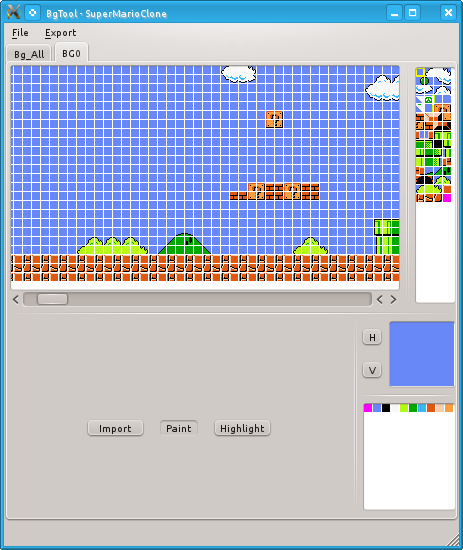
\includegraphics{imgs/bgtool2.png}
\caption{Apagando os objetos depois de importar a imagem.} 
\end{figure}

Começamos importando uma imagem da primeira fase do jogo original na BGTool, criando um mapa da primeira fase, e editamos o mapa para retirar objetos que não são do background, como as caixas de interrogação. E usamos a ferramenta para exportar para o DS. Repetimos esse processo para as fases que incluímos neste nosso jogo de demonstração.



\chapter{Conclusões e trabalhos futuros\label{cap:conclusao}}

\vfill{}
\begin{flushright}{}``\emph{Nada se cria, nada se perde, tudo se
transforma.}''\\
{\small Lavousier}\end{flushright}{\small \par}
\vfill{}

Neste capítulo é apresentado as conclusões e alguns trabalhos futuros
...
\newpage


\section{Conclusões}

O mercado de jogos está finalmente chegando em sua maturidade. Jogos feitos por pequenos grupos de desenvolvedores estão alcançando sucesso tão grande quanto grandes franquias, criadas por grandes empresas. Como exemplo disso, podem-se citar jogos como Minecraft, que foi desenvolvido por boa parte do tempo por apenas um desenvolvedor, que há pouco tempo alcançou a marca de mais de 2 milhões de cópias vendidas. \cite{MinecraftSales}

Com esse cenário, podemos notar que é importante tentar reduzir o tempo gasto mexendo em código fonte, para que os desenvolvedores possam se focar naquilo que realmente faz diferença em um jogo: a originalidade e o seu \textit{gameplay}.

A maior dificuldade nesse tipo de projeto, como citado anteriormente, é o acesso às funções de hardware dos consoles. Entretanto, é possível perceber um movimento das grandes empresas em direção a consoles com desenvolvimento mais aberto, como por exemplo o Xbox Live Indie Games, onde o desenvolvedor usa o XNA Game Studio para desenvolver e recebe 70\% do lucro do lançamento do seu jogo, depois de alguns passos que conferem ao jogo a possibilidade de ser lançado. Ainda assim, há um custo anual para o desenvolvedor de \$99 USD. \cite{XNAAppHub} 

As ferramentas desenvolvidas nesse trabalho tem como objetivo ser apenas uma idéia do que os autores pensam ser um caminho para reduzir esse gasto, fazendo com que seja possível desenvolver jogos bem diferentes com pequenas alterações de código. Embora com essas ferramentas não seja possível publicar um jogo, há a possibilidade de um desenvolvedor individual as utilizar para desenvolver um protótipo de jogo, ou para um jogo que não tenha intenção de ser vendido na plataforma.

Podemos dizer que ainda há muito a ser feito para essas ferramentas. Poderíamos, por exemplo, escrever mais funções que exportem para diferentes cadeias de ferramentas, de diferentes sistemas. Não nos limitando, então, somente ao Nintendo DS. Deste modo, poderia ser desenvolvido um jogo de diversas plataformas com um mínimo de trabalho.

Além disso, certas tarefas podem ser mais automatizadas, como a geração do arquivo que carrega os \textit{backgrounds} e personagens na \textit{engine} do DS. Como tem um formato bem definido, ele poderia ser gerado automaticamente por uma terceira ferramenta que conseguisse ler o formato XML definido neste trabalho.

%Caso a gente termine a interface da colisão, tirar isso daqui

A colisão precisa ser definida manualmente na \textit{engine}, mas isso poderia ser feito diretamente na BGTool, ao importar os \textit{tiles}. Assim, o artista que estivesse criando os \textit{backgrounds} poderia já escolher o tipo de colisão dos seus trabalhos.

A interface da BGTool ainda pode ser melhorada, para facilitar o seu uso. Com operações de pintura em grupo, preenchimento de regiões por difusão (flood-fill), e outras operações comuns em ferramentas de desenho.

\bibliographystyle{abnt-alf}
\bibliography{PF}


\anexo

\chapter{Ferramentas utilizadas}

\section{QT}


\end{document}
